\chapter{Kết quả \& Thảo luận}
\label{Chapter5}

\section{Đánh giá mô hình Medicine Classifier}

Medicine Classifier là một bước quan trọng trong phương pháp đề xuất \codeword{MEP} của chúng tôi. Nếu như nó hoạt động không hiệu quả thì hệ thống nhận diện đơn thuốc cũng sẽ không thể sử dụng được.

Theo như phần huấn luyện mô hình, Medicine Classifier hội tụ nhanh và chỉ trong vòng 20 epoch đã đạt được cực tiểu cho hàm $loss$. Hình ~\ref{tfw_acc}, ~\ref{tfw_loss}, ~\ref{tfw_precision}, ~\ref{tfw_recall} thể hiện kết quả huấn luyện cho mô hình Medicine Classifier, được theo dõi và thống kê bằng TF Watcher \cite{TFWatcher}. 

\begin{figure}
\centering
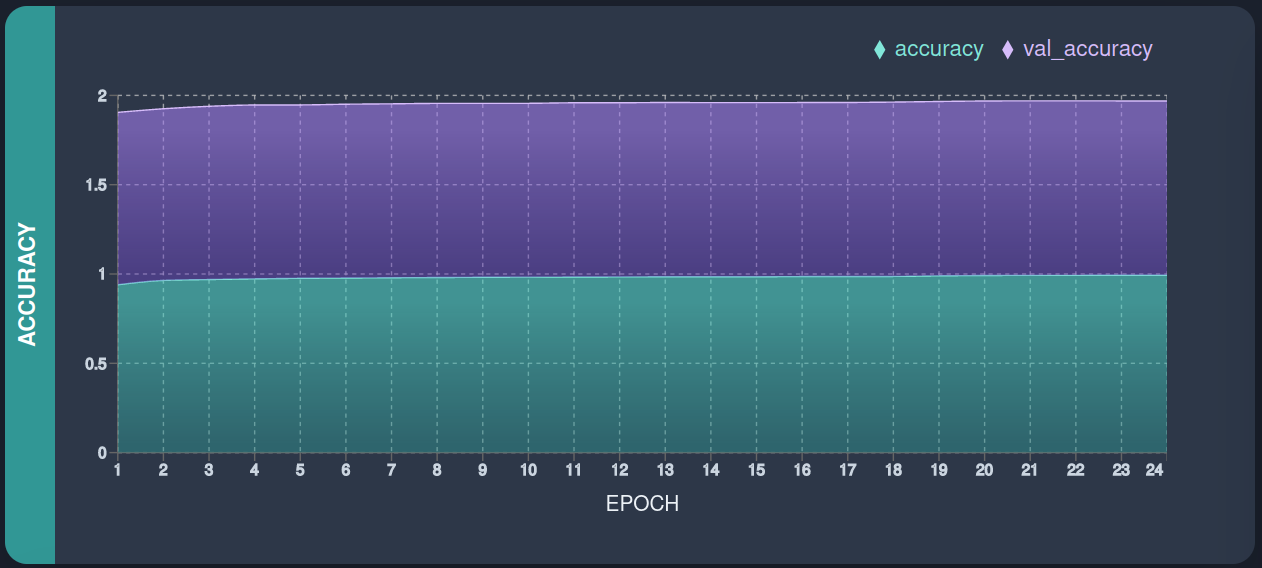
\includegraphics[width=0.8\textwidth]{mep_img/tfw_acc.png}
\caption{Độ chính xác của mô hình Medicine Classifier trong quá trình huấn luyện.}\label{tfw_acc}
\end{figure}

\begin{figure}
\centering
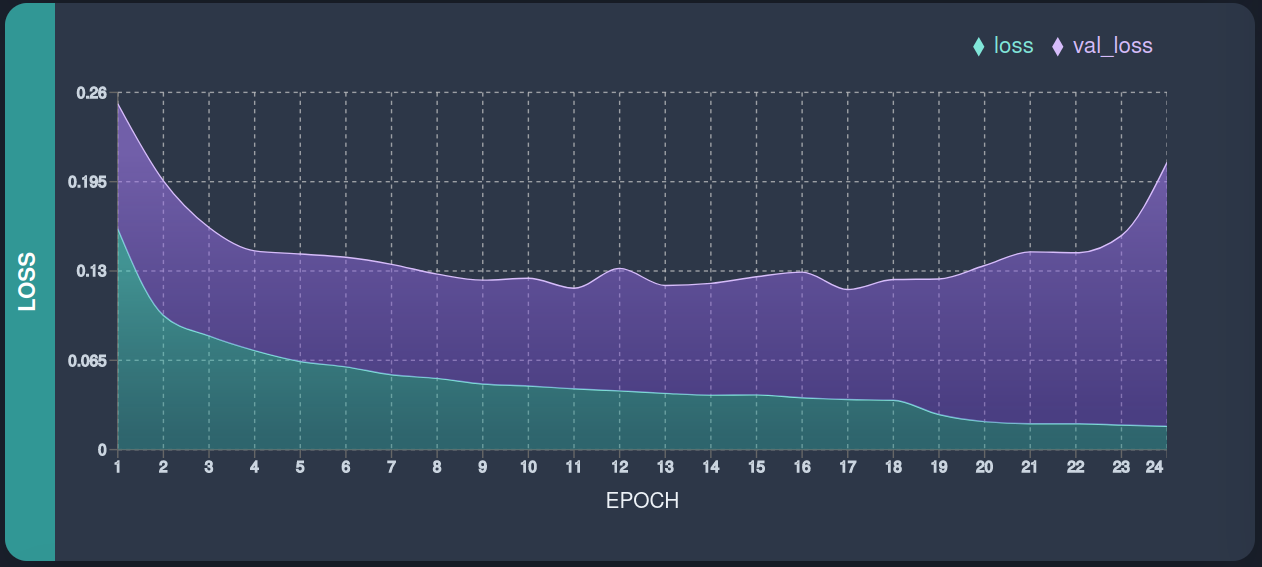
\includegraphics[width=0.8\textwidth]{mep_img/tfw_loss.png}
\caption{Hàm lỗi của mô hình Medicine Classifier trong quá trình huấn luyện.}\label{tfw_loss}
\end{figure}

\begin{figure}
\centering
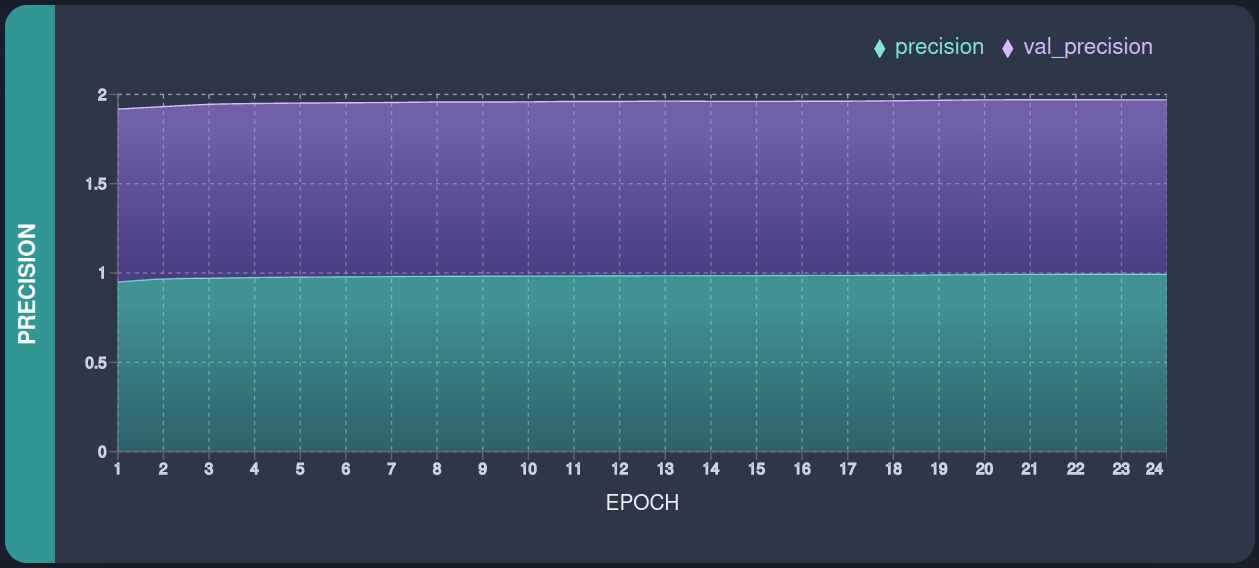
\includegraphics[width=0.8\textwidth]{mep_img/tfw_precision.png}
\caption{Đánh giá mô hình Medicine Classifier bằng độ đo precision trong quá trình huấn luyện.}\label{tfw_precision}
\end{figure}

\begin{figure}
\centering
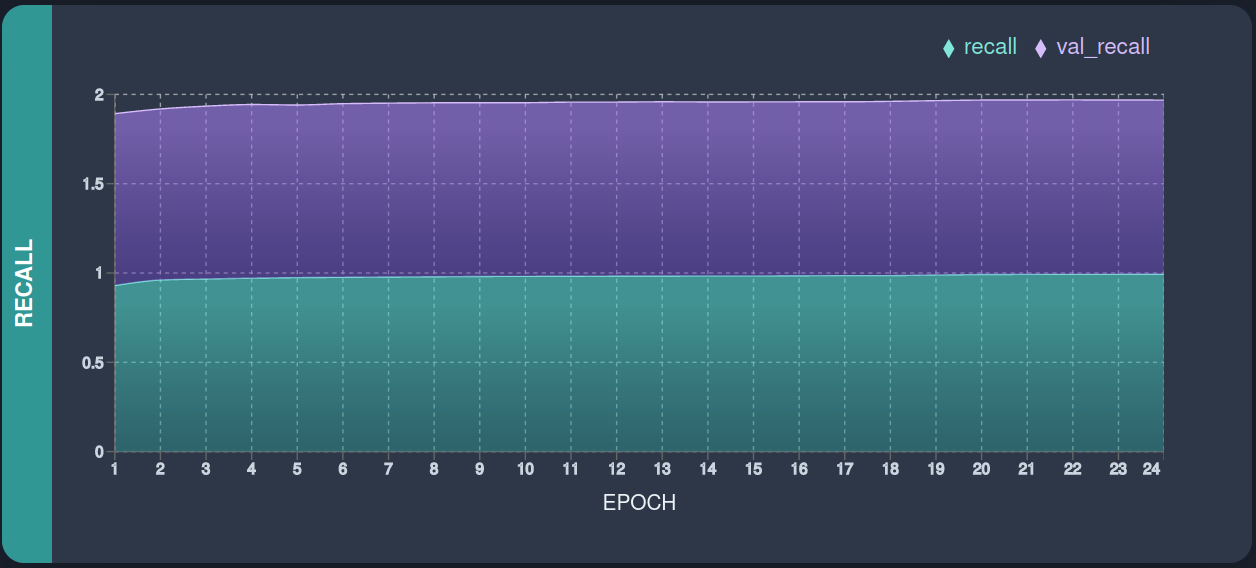
\includegraphics[width=0.8\textwidth]{mep_img/tfw_recall.png}
\caption{Đánh giá mô hình Medicine Classifier bằng độ đo recall trong quá trình huấn luyện.}\label{tfw_recall}
\end{figure}

Từ kết quả trên, ta nhanh chóng nhận ra cả 3 độ đo Accuracy \textit{acc}, Precision \textit{P}, và Recall \textit{R} đều nhanh chóng hội tụ và rất cao, chứng tỏ mô hình này rất phù hợp với bộ dữ liệu cũng như bài toán đặt ra. Các thông số trên đều cao trên $0.95$ khi đánh giá trên cả tập $D_{train}$ lẫn tập $D_{validation}$.

Đối với hàm \textit{loss}, chúng tôi quan sát và thấy rằng ban đầu, cả 2 hàm $L_{train}$ và $L_{validation}$ cho 2 tập đều thấp, với $L_{train} = 0.16$ và $L_{validation} = 0.09$. Những hàm \textit{loss} này giảm dần đều và có sự hoán đổi về mặt giá trị giữa 2 hàm trong trong quá trình huấn luyện mô hình. 

Cực tiểu của hàm $L_{validation}$ là tại \verb|epoch = 11|. Tuy nhiên, khi đến \verb|epoch = 18|, mô hình có dấu hiệu bị overfit, làm $L_{train}$ giảm nhanh nhưng hàm $L_{validation}$ thì lại tăng đáng kể. Vì vậy, chúng tôi chọn checkpoint tốt nhất để sử dụng cho \codeword{MEP} tại epoch bằng 11.

Mô hình Medicine Classifier sau khi được huấn luyện cho kết quả khả quan, đạt $acc_{test} = 0.97$ và $L_{test} = 0.11$ khi đánh giá trên tập ẩn $D_{test}$.

\section{Đánh giá độ chính xác của phương pháp đề xuất MEP}

Chúng tôi thực hiện chạy thử nghiệm trên tập dữ liệu đơn thuốc mà chúng tôi thu thập, được giới thiệu tại mục Chương 4 trên cả hai mô hình, gồm mô hình đề xuất \codeword{MEP} và mô hình tại \cite{nguyen2021developing}.

Bảng ~\ref{exp:tab_1} thể hiện kết quả của \codeword{MEP} so với hệ thống cũ. 

\begin{table}
\centering
\caption{Đánh giá kết quả của hai mô hình nhận dạng đơn thuốc, gồm \textbf{MEP} và \cite{nguyen2021developing}}\label{exp:tab_1}
% \begin{tabular}{|S[table-format=15.0]|S[table-format=10.2]|S[table-format=7.2]|S[table-format=7.2]|}
\begin{tabular}{|c|ccc|}
\hline
Model           & @Precision & @Recall & @H-mean  \\ 
\hline
Method in \cite{nguyen2021developing}      & 0.54       & 0.17    & 0.26     \\ 
\hline
\textbf{MEP} & \textbf{0.94}       & \textbf{0.73}    & \textbf{0.82}     \\
\hline
\end{tabular}
\end{table}

Có thể thấy, các chỉ số độ đo của \codeword{MEP} đều cao hơn hẳn so với mô hình trước đó. Độ đo precision $P_{MEP}$ lên tới \textbf{0.94}, tăng thêm \textbf{0.4} so với phiên bản tiền nghiệm. Điều đó cho thấy, hầu hết trong số các tên thuốc mà mô hình chúng tôi nhận dạng được thì đều đảm bảo độ chính xác. 

Mặc dù thông số recall $R_{MEP}$ tăng rất ấn tượng, cách biệt \textbf{0.54} so với phiên bản tiền nghiệm, tuy nhiên nó mới chỉ đạt \textbf{0.73} cho toàn bộ tập dữ liệu kiểm thử. Điều này có thể là do đầu vào của mô hình bao gồm các đơn thuốc có nhiều nhiễu, dẫn đến OCR chưa lấy được đầy đủ văn bản để mô hình thực hiện trích xuất tên thuốc.

Một nguyên nhân nữa cũng ảnh hưởng đến kết quả của $R_{MEP}$ đó là công đoạn Medicine Extractor vì các tên thuốc tiềm năng được trích xuất ra dựa rất nhiều vào công đoạn này. Mặc dù phần lớn đơn thuốc sẽ thuộc về 2 trường hợp mà chúng tôi đang khai thác, vẫn có một lượng dữ liệu đơn thuốc không theo chuẩn này dẫn đến khó khăn cho mô hình. Điều này hoàn toàn có thể được cải thiện trong những phiên bản tới, khi chúng tôi tăng cường nhiều luật hơn cho Medicine Extractor.

\begin{table}
\centering
\caption{Tầm quan trọng của Medicine Extractor trong hệ thống nhận dạng đơn thuốc}\label{exp:tab_2}
% \begin{tabular}{|S[table-format=15.0]|S[table-format=10.2]|S[table-format=7.2]|S[table-format=7.2]|}
\begin{adjustbox}{angle=-90}
\begin{tabular}{|c|c|c|c|c|}
\hline
Model           & OCRed text & MedicineExtractor & Spell correction & Output \\ 
\hline
Method in \cite{nguyen2021developing}      & Allpovic & - & [Alpovic]@0.9 & Alpovic     \\ 
\textbf{MEP} & Allpovic & \textbf{Allpovic} & [Alpovic]@0.9 & Alpovic     \\
\hline
Method in \cite{nguyen2021developing}      & Eperison 50mg (Macnir) & - & [Macnir]@0.6 & -      \\ 
\textbf{MEP} & Eperison 50mg (Macnir) & \textbf{Macnir} & [Macnir]@1.0 & Macnir     \\
\hline
\textbf{MEP} & Diovan 160mg (Valsartan) & \textbf{Diovan 160mg} & [Diovan 160]@0.94 & Diovan 160     \\
\hline
\end{tabular}
\end{adjustbox}
\end{table}

Ngoài ra, bảng ~\ref{exp:tab_2} cũng chỉ ra tại sao mô hình của chúng tôi hoạt động ổn định hơn phiên bản tiền nghiệm. Chúng tôi giả sử hệ thống OCR làm việc tích cực và cho ra kết quả tương đối chính xác trên cả 2 mô hình, mặc dù điều này là khó đạt được tại \cite{nguyen2021developing} trong bối cảnh sử dụng Tesseract làm bộ nhận dạng văn bản. Đối với văn bản được trích xuất là "Allpovic", cả hai hệ thống trích xuất tên thuốc hoạt động tốt khi độ tin cậy của kết quả trả ra lên tới \textbf{0.9}, mặc dù tên thuốc này đang là sai chính tả.

Tuy nhiên, sự khác biệt bắt đầu xảy ra khi văn bản sau bước OCR là "Eperison 50mg (Macnir)". Việc chỉ so khớp với từ điển thuốc đã khiến cho độ tin cậy của kết quả tại mô hình \cite{nguyen2021developing} bị sụt giảm nghiêm trọng, tụt xuống \textbf{0.6}, thấp hơn ngưỡng mà mô hình sử dụng. Điều đó dẫn đến nó không thể phát hiện đây là tên thuốc, và cũng là một trong những nguyên nhân khiến cho \textit{Recall} của mô hình này chỉ đạt 0.17.

\codeword{MEP} có thể giải quyết được vấn đề này một cách triệt để khi Medicine Extractor có thể tách thông tin trong input này ra, một là “Epersion 50mg”, còn lại là "Macnir". "Epersion 50mg" là hoạt chất, nên tất nhiên sẽ được loại bỏ ở những bước phía sau, còn "Macnir" sẽ được đánh dấu là tên thuốc với độ tin cậy tuyệt đối. Tương tự với trường hợp thứ 3, khi thứ tự giữa tên thuốc và hoạt chất trong văn bản sau bước OCR có sự thay đổi, các luật của mô hình chúng tôi vẫn đảm bảo sự ổn định cho kết quả tổng quan của mô hình.

\section{Đánh giá hiệu suất của mô hình}

Ngoài tiêu chí về độ chính xác, thời gian thực thi cũng là một yếu tố quan trọng quyết định đến một mô hình có được ưu tiên sử dụng hay không. Một mô hình với kết quả tuyệt đối nhưng lại mất nhiều thời gian xử lý và tốn nhiều tài nguyên thường không được sử dụng trong thực tế và đem lại giá trị.

Cơ bản, chúng ta cũng biết phần cứng của máy tính mặc dù được mở rộng trong những năm gần đây, tuy nhiên cũng không đủ đáp ứng nếu như không có sự tối ưu đến từ cả hai phía. Mô hình nhận diện tên thuốc do chúng tôi đề xuất được cấu tạo từ nhiều phần, với mỗi phần mang một sứ mệnh khác nhau. Vì vậy, chúng tôi muốn chứng minh rằng các phần này không tỉ lệ thuận với thời gian thực thi và đưa ra kết quả. Cụ thể, kết quả đo lường trên từng công đoạn của mô hình được so sánh và chỉ ra trong hình ~\ref{exp:barchart}.

\begin{figure}
\centering
\scalebox{0.65}{%% Creator: Matplotlib, PGF backend
%%
%% To include the figure in your LaTeX document, write
%%   \input{<filename>.pgf}
%%
%% Make sure the required packages are loaded in your preamble
%%   \usepackage{pgf}
%%
%% Also ensure that all the required font packages are loaded; for instance,
%% the lmodern package is sometimes necessary when using math font.
%%   \usepackage{lmodern}
%%
%% Figures using additional raster images can only be included by \input if
%% they are in the same directory as the main LaTeX file. For loading figures
%% from other directories you can use the `import` package
%%   \usepackage{import}
%%
%% and then include the figures with
%%   \import{<path to file>}{<filename>.pgf}
%%
%% Matplotlib used the following preamble
%%
\begingroup%
\makeatletter%
\begin{pgfpicture}%
\pgfpathrectangle{\pgfpointorigin}{\pgfqpoint{9.000000in}{5.000000in}}%
\pgfusepath{use as bounding box, clip}%
\begin{pgfscope}%
\pgfsetbuttcap%
\pgfsetmiterjoin%
\pgfsetlinewidth{0.000000pt}%
\definecolor{currentstroke}{rgb}{1.000000,1.000000,1.000000}%
\pgfsetstrokecolor{currentstroke}%
\pgfsetstrokeopacity{0.000000}%
\pgfsetdash{}{0pt}%
\pgfpathmoveto{\pgfqpoint{0.000000in}{0.000000in}}%
\pgfpathlineto{\pgfqpoint{9.000000in}{0.000000in}}%
\pgfpathlineto{\pgfqpoint{9.000000in}{5.000000in}}%
\pgfpathlineto{\pgfqpoint{0.000000in}{5.000000in}}%
\pgfpathlineto{\pgfqpoint{0.000000in}{0.000000in}}%
\pgfpathclose%
\pgfusepath{}%
\end{pgfscope}%
\begin{pgfscope}%
\pgfsetbuttcap%
\pgfsetmiterjoin%
\definecolor{currentfill}{rgb}{1.000000,1.000000,1.000000}%
\pgfsetfillcolor{currentfill}%
\pgfsetlinewidth{0.000000pt}%
\definecolor{currentstroke}{rgb}{0.000000,0.000000,0.000000}%
\pgfsetstrokecolor{currentstroke}%
\pgfsetstrokeopacity{0.000000}%
\pgfsetdash{}{0pt}%
\pgfpathmoveto{\pgfqpoint{0.516436in}{0.264771in}}%
\pgfpathlineto{\pgfqpoint{8.887500in}{0.264771in}}%
\pgfpathlineto{\pgfqpoint{8.887500in}{4.750662in}}%
\pgfpathlineto{\pgfqpoint{0.516436in}{4.750662in}}%
\pgfpathlineto{\pgfqpoint{0.516436in}{0.264771in}}%
\pgfpathclose%
\pgfusepath{fill}%
\end{pgfscope}%
\begin{pgfscope}%
\pgfpathrectangle{\pgfqpoint{0.516436in}{0.264771in}}{\pgfqpoint{8.371064in}{4.485891in}}%
\pgfusepath{clip}%
\pgfsetbuttcap%
\pgfsetmiterjoin%
\definecolor{currentfill}{rgb}{0.121569,0.466667,0.705882}%
\pgfsetfillcolor{currentfill}%
\pgfsetlinewidth{0.000000pt}%
\definecolor{currentstroke}{rgb}{0.000000,0.000000,0.000000}%
\pgfsetstrokecolor{currentstroke}%
\pgfsetstrokeopacity{0.000000}%
\pgfsetdash{}{0pt}%
\pgfpathmoveto{\pgfqpoint{0.896939in}{0.264771in}}%
\pgfpathlineto{\pgfqpoint{1.242850in}{0.264771in}}%
\pgfpathlineto{\pgfqpoint{1.242850in}{0.368763in}}%
\pgfpathlineto{\pgfqpoint{0.896939in}{0.368763in}}%
\pgfpathlineto{\pgfqpoint{0.896939in}{0.264771in}}%
\pgfpathclose%
\pgfusepath{fill}%
\end{pgfscope}%
\begin{pgfscope}%
\pgfpathrectangle{\pgfqpoint{0.516436in}{0.264771in}}{\pgfqpoint{8.371064in}{4.485891in}}%
\pgfusepath{clip}%
\pgfsetbuttcap%
\pgfsetmiterjoin%
\definecolor{currentfill}{rgb}{0.121569,0.466667,0.705882}%
\pgfsetfillcolor{currentfill}%
\pgfsetlinewidth{0.000000pt}%
\definecolor{currentstroke}{rgb}{0.000000,0.000000,0.000000}%
\pgfsetstrokecolor{currentstroke}%
\pgfsetstrokeopacity{0.000000}%
\pgfsetdash{}{0pt}%
\pgfpathmoveto{\pgfqpoint{1.885258in}{0.264771in}}%
\pgfpathlineto{\pgfqpoint{2.231170in}{0.264771in}}%
\pgfpathlineto{\pgfqpoint{2.231170in}{4.064071in}}%
\pgfpathlineto{\pgfqpoint{1.885258in}{4.064071in}}%
\pgfpathlineto{\pgfqpoint{1.885258in}{0.264771in}}%
\pgfpathclose%
\pgfusepath{fill}%
\end{pgfscope}%
\begin{pgfscope}%
\pgfpathrectangle{\pgfqpoint{0.516436in}{0.264771in}}{\pgfqpoint{8.371064in}{4.485891in}}%
\pgfusepath{clip}%
\pgfsetbuttcap%
\pgfsetmiterjoin%
\definecolor{currentfill}{rgb}{0.121569,0.466667,0.705882}%
\pgfsetfillcolor{currentfill}%
\pgfsetlinewidth{0.000000pt}%
\definecolor{currentstroke}{rgb}{0.000000,0.000000,0.000000}%
\pgfsetstrokecolor{currentstroke}%
\pgfsetstrokeopacity{0.000000}%
\pgfsetdash{}{0pt}%
\pgfpathmoveto{\pgfqpoint{2.873577in}{0.264771in}}%
\pgfpathlineto{\pgfqpoint{3.219489in}{0.264771in}}%
\pgfpathlineto{\pgfqpoint{3.219489in}{0.633754in}}%
\pgfpathlineto{\pgfqpoint{2.873577in}{0.633754in}}%
\pgfpathlineto{\pgfqpoint{2.873577in}{0.264771in}}%
\pgfpathclose%
\pgfusepath{fill}%
\end{pgfscope}%
\begin{pgfscope}%
\pgfpathrectangle{\pgfqpoint{0.516436in}{0.264771in}}{\pgfqpoint{8.371064in}{4.485891in}}%
\pgfusepath{clip}%
\pgfsetbuttcap%
\pgfsetmiterjoin%
\definecolor{currentfill}{rgb}{0.121569,0.466667,0.705882}%
\pgfsetfillcolor{currentfill}%
\pgfsetlinewidth{0.000000pt}%
\definecolor{currentstroke}{rgb}{0.000000,0.000000,0.000000}%
\pgfsetstrokecolor{currentstroke}%
\pgfsetstrokeopacity{0.000000}%
\pgfsetdash{}{0pt}%
\pgfpathmoveto{\pgfqpoint{3.861896in}{0.264771in}}%
\pgfpathlineto{\pgfqpoint{4.207808in}{0.264771in}}%
\pgfpathlineto{\pgfqpoint{4.207808in}{4.537048in}}%
\pgfpathlineto{\pgfqpoint{3.861896in}{4.537048in}}%
\pgfpathlineto{\pgfqpoint{3.861896in}{0.264771in}}%
\pgfpathclose%
\pgfusepath{fill}%
\end{pgfscope}%
\begin{pgfscope}%
\pgfpathrectangle{\pgfqpoint{0.516436in}{0.264771in}}{\pgfqpoint{8.371064in}{4.485891in}}%
\pgfusepath{clip}%
\pgfsetbuttcap%
\pgfsetmiterjoin%
\definecolor{currentfill}{rgb}{1.000000,0.498039,0.054902}%
\pgfsetfillcolor{currentfill}%
\pgfsetlinewidth{0.000000pt}%
\definecolor{currentstroke}{rgb}{0.000000,0.000000,0.000000}%
\pgfsetstrokecolor{currentstroke}%
\pgfsetstrokeopacity{0.000000}%
\pgfsetdash{}{0pt}%
\pgfpathmoveto{\pgfqpoint{1.242850in}{0.264771in}}%
\pgfpathlineto{\pgfqpoint{1.588762in}{0.264771in}}%
\pgfpathlineto{\pgfqpoint{1.588762in}{0.569467in}}%
\pgfpathlineto{\pgfqpoint{1.242850in}{0.569467in}}%
\pgfpathlineto{\pgfqpoint{1.242850in}{0.264771in}}%
\pgfpathclose%
\pgfusepath{fill}%
\end{pgfscope}%
\begin{pgfscope}%
\pgfpathrectangle{\pgfqpoint{0.516436in}{0.264771in}}{\pgfqpoint{8.371064in}{4.485891in}}%
\pgfusepath{clip}%
\pgfsetbuttcap%
\pgfsetmiterjoin%
\definecolor{currentfill}{rgb}{1.000000,0.498039,0.054902}%
\pgfsetfillcolor{currentfill}%
\pgfsetlinewidth{0.000000pt}%
\definecolor{currentstroke}{rgb}{0.000000,0.000000,0.000000}%
\pgfsetstrokecolor{currentstroke}%
\pgfsetstrokeopacity{0.000000}%
\pgfsetdash{}{0pt}%
\pgfpathmoveto{\pgfqpoint{2.231170in}{0.264771in}}%
\pgfpathlineto{\pgfqpoint{2.577081in}{0.264771in}}%
\pgfpathlineto{\pgfqpoint{2.577081in}{0.658542in}}%
\pgfpathlineto{\pgfqpoint{2.231170in}{0.658542in}}%
\pgfpathlineto{\pgfqpoint{2.231170in}{0.264771in}}%
\pgfpathclose%
\pgfusepath{fill}%
\end{pgfscope}%
\begin{pgfscope}%
\pgfpathrectangle{\pgfqpoint{0.516436in}{0.264771in}}{\pgfqpoint{8.371064in}{4.485891in}}%
\pgfusepath{clip}%
\pgfsetbuttcap%
\pgfsetmiterjoin%
\definecolor{currentfill}{rgb}{1.000000,0.498039,0.054902}%
\pgfsetfillcolor{currentfill}%
\pgfsetlinewidth{0.000000pt}%
\definecolor{currentstroke}{rgb}{0.000000,0.000000,0.000000}%
\pgfsetstrokecolor{currentstroke}%
\pgfsetstrokeopacity{0.000000}%
\pgfsetdash{}{0pt}%
\pgfpathmoveto{\pgfqpoint{3.219489in}{0.264771in}}%
\pgfpathlineto{\pgfqpoint{3.565401in}{0.264771in}}%
\pgfpathlineto{\pgfqpoint{3.565401in}{1.040398in}}%
\pgfpathlineto{\pgfqpoint{3.219489in}{1.040398in}}%
\pgfpathlineto{\pgfqpoint{3.219489in}{0.264771in}}%
\pgfpathclose%
\pgfusepath{fill}%
\end{pgfscope}%
\begin{pgfscope}%
\pgfpathrectangle{\pgfqpoint{0.516436in}{0.264771in}}{\pgfqpoint{8.371064in}{4.485891in}}%
\pgfusepath{clip}%
\pgfsetbuttcap%
\pgfsetmiterjoin%
\definecolor{currentfill}{rgb}{1.000000,0.498039,0.054902}%
\pgfsetfillcolor{currentfill}%
\pgfsetlinewidth{0.000000pt}%
\definecolor{currentstroke}{rgb}{0.000000,0.000000,0.000000}%
\pgfsetstrokecolor{currentstroke}%
\pgfsetstrokeopacity{0.000000}%
\pgfsetdash{}{0pt}%
\pgfpathmoveto{\pgfqpoint{4.207808in}{0.264771in}}%
\pgfpathlineto{\pgfqpoint{4.553720in}{0.264771in}}%
\pgfpathlineto{\pgfqpoint{4.553720in}{1.863732in}}%
\pgfpathlineto{\pgfqpoint{4.207808in}{1.863732in}}%
\pgfpathlineto{\pgfqpoint{4.207808in}{0.264771in}}%
\pgfpathclose%
\pgfusepath{fill}%
\end{pgfscope}%
\begin{pgfscope}%
\pgfpathrectangle{\pgfqpoint{0.516436in}{0.264771in}}{\pgfqpoint{8.371064in}{4.485891in}}%
\pgfusepath{clip}%
\pgfsetbuttcap%
\pgfsetmiterjoin%
\definecolor{currentfill}{rgb}{1.000000,0.498039,0.054902}%
\pgfsetfillcolor{currentfill}%
\pgfsetlinewidth{0.000000pt}%
\definecolor{currentstroke}{rgb}{0.000000,0.000000,0.000000}%
\pgfsetstrokecolor{currentstroke}%
\pgfsetstrokeopacity{0.000000}%
\pgfsetdash{}{0pt}%
\pgfpathmoveto{\pgfqpoint{5.196128in}{0.264771in}}%
\pgfpathlineto{\pgfqpoint{5.542039in}{0.264771in}}%
\pgfpathlineto{\pgfqpoint{5.542039in}{0.388995in}}%
\pgfpathlineto{\pgfqpoint{5.196128in}{0.388995in}}%
\pgfpathlineto{\pgfqpoint{5.196128in}{0.264771in}}%
\pgfpathclose%
\pgfusepath{fill}%
\end{pgfscope}%
\begin{pgfscope}%
\pgfpathrectangle{\pgfqpoint{0.516436in}{0.264771in}}{\pgfqpoint{8.371064in}{4.485891in}}%
\pgfusepath{clip}%
\pgfsetbuttcap%
\pgfsetmiterjoin%
\definecolor{currentfill}{rgb}{1.000000,0.498039,0.054902}%
\pgfsetfillcolor{currentfill}%
\pgfsetlinewidth{0.000000pt}%
\definecolor{currentstroke}{rgb}{0.000000,0.000000,0.000000}%
\pgfsetstrokecolor{currentstroke}%
\pgfsetstrokeopacity{0.000000}%
\pgfsetdash{}{0pt}%
\pgfpathmoveto{\pgfqpoint{6.184447in}{0.264771in}}%
\pgfpathlineto{\pgfqpoint{6.530359in}{0.264771in}}%
\pgfpathlineto{\pgfqpoint{6.530359in}{0.264804in}}%
\pgfpathlineto{\pgfqpoint{6.184447in}{0.264804in}}%
\pgfpathlineto{\pgfqpoint{6.184447in}{0.264771in}}%
\pgfpathclose%
\pgfusepath{fill}%
\end{pgfscope}%
\begin{pgfscope}%
\pgfpathrectangle{\pgfqpoint{0.516436in}{0.264771in}}{\pgfqpoint{8.371064in}{4.485891in}}%
\pgfusepath{clip}%
\pgfsetbuttcap%
\pgfsetmiterjoin%
\definecolor{currentfill}{rgb}{1.000000,0.498039,0.054902}%
\pgfsetfillcolor{currentfill}%
\pgfsetlinewidth{0.000000pt}%
\definecolor{currentstroke}{rgb}{0.000000,0.000000,0.000000}%
\pgfsetstrokecolor{currentstroke}%
\pgfsetstrokeopacity{0.000000}%
\pgfsetdash{}{0pt}%
\pgfpathmoveto{\pgfqpoint{7.172766in}{0.264771in}}%
\pgfpathlineto{\pgfqpoint{7.518678in}{0.264771in}}%
\pgfpathlineto{\pgfqpoint{7.518678in}{0.356353in}}%
\pgfpathlineto{\pgfqpoint{7.172766in}{0.356353in}}%
\pgfpathlineto{\pgfqpoint{7.172766in}{0.264771in}}%
\pgfpathclose%
\pgfusepath{fill}%
\end{pgfscope}%
\begin{pgfscope}%
\pgfpathrectangle{\pgfqpoint{0.516436in}{0.264771in}}{\pgfqpoint{8.371064in}{4.485891in}}%
\pgfusepath{clip}%
\pgfsetbuttcap%
\pgfsetmiterjoin%
\definecolor{currentfill}{rgb}{1.000000,0.498039,0.054902}%
\pgfsetfillcolor{currentfill}%
\pgfsetlinewidth{0.000000pt}%
\definecolor{currentstroke}{rgb}{0.000000,0.000000,0.000000}%
\pgfsetstrokecolor{currentstroke}%
\pgfsetstrokeopacity{0.000000}%
\pgfsetdash{}{0pt}%
\pgfpathmoveto{\pgfqpoint{8.161085in}{0.264771in}}%
\pgfpathlineto{\pgfqpoint{8.506997in}{0.264771in}}%
\pgfpathlineto{\pgfqpoint{8.506997in}{0.959016in}}%
\pgfpathlineto{\pgfqpoint{8.161085in}{0.959016in}}%
\pgfpathlineto{\pgfqpoint{8.161085in}{0.264771in}}%
\pgfpathclose%
\pgfusepath{fill}%
\end{pgfscope}%
\begin{pgfscope}%
\pgfsetbuttcap%
\pgfsetroundjoin%
\definecolor{currentfill}{rgb}{0.000000,0.000000,0.000000}%
\pgfsetfillcolor{currentfill}%
\pgfsetlinewidth{0.803000pt}%
\definecolor{currentstroke}{rgb}{0.000000,0.000000,0.000000}%
\pgfsetstrokecolor{currentstroke}%
\pgfsetdash{}{0pt}%
\pgfsys@defobject{currentmarker}{\pgfqpoint{0.000000in}{-0.048611in}}{\pgfqpoint{0.000000in}{0.000000in}}{%
\pgfpathmoveto{\pgfqpoint{0.000000in}{0.000000in}}%
\pgfpathlineto{\pgfqpoint{0.000000in}{-0.048611in}}%
\pgfusepath{stroke,fill}%
}%
\begin{pgfscope}%
\pgfsys@transformshift{1.242850in}{0.264771in}%
\pgfsys@useobject{currentmarker}{}%
\end{pgfscope}%
\end{pgfscope}%
\begin{pgfscope}%
\definecolor{textcolor}{rgb}{0.000000,0.000000,0.000000}%
\pgfsetstrokecolor{textcolor}%
\pgfsetfillcolor{textcolor}%
\pgftext[x=1.242850in,y=0.167548in,,top]{\color{textcolor}\rmfamily\fontsize{10.000000}{12.000000}\selectfont detection}%
\end{pgfscope}%
\begin{pgfscope}%
\pgfsetbuttcap%
\pgfsetroundjoin%
\definecolor{currentfill}{rgb}{0.000000,0.000000,0.000000}%
\pgfsetfillcolor{currentfill}%
\pgfsetlinewidth{0.803000pt}%
\definecolor{currentstroke}{rgb}{0.000000,0.000000,0.000000}%
\pgfsetstrokecolor{currentstroke}%
\pgfsetdash{}{0pt}%
\pgfsys@defobject{currentmarker}{\pgfqpoint{0.000000in}{-0.048611in}}{\pgfqpoint{0.000000in}{0.000000in}}{%
\pgfpathmoveto{\pgfqpoint{0.000000in}{0.000000in}}%
\pgfpathlineto{\pgfqpoint{0.000000in}{-0.048611in}}%
\pgfusepath{stroke,fill}%
}%
\begin{pgfscope}%
\pgfsys@transformshift{2.231170in}{0.264771in}%
\pgfsys@useobject{currentmarker}{}%
\end{pgfscope}%
\end{pgfscope}%
\begin{pgfscope}%
\definecolor{textcolor}{rgb}{0.000000,0.000000,0.000000}%
\pgfsetstrokecolor{textcolor}%
\pgfsetfillcolor{textcolor}%
\pgftext[x=2.231170in,y=0.167548in,,top]{\color{textcolor}\rmfamily\fontsize{10.000000}{12.000000}\selectfont recognition}%
\end{pgfscope}%
\begin{pgfscope}%
\pgfsetbuttcap%
\pgfsetroundjoin%
\definecolor{currentfill}{rgb}{0.000000,0.000000,0.000000}%
\pgfsetfillcolor{currentfill}%
\pgfsetlinewidth{0.803000pt}%
\definecolor{currentstroke}{rgb}{0.000000,0.000000,0.000000}%
\pgfsetstrokecolor{currentstroke}%
\pgfsetdash{}{0pt}%
\pgfsys@defobject{currentmarker}{\pgfqpoint{0.000000in}{-0.048611in}}{\pgfqpoint{0.000000in}{0.000000in}}{%
\pgfpathmoveto{\pgfqpoint{0.000000in}{0.000000in}}%
\pgfpathlineto{\pgfqpoint{0.000000in}{-0.048611in}}%
\pgfusepath{stroke,fill}%
}%
\begin{pgfscope}%
\pgfsys@transformshift{3.219489in}{0.264771in}%
\pgfsys@useobject{currentmarker}{}%
\end{pgfscope}%
\end{pgfscope}%
\begin{pgfscope}%
\definecolor{textcolor}{rgb}{0.000000,0.000000,0.000000}%
\pgfsetstrokecolor{textcolor}%
\pgfsetfillcolor{textcolor}%
\pgftext[x=3.219489in,y=0.167548in,,top]{\color{textcolor}\rmfamily\fontsize{10.000000}{12.000000}\selectfont recorrect}%
\end{pgfscope}%
\begin{pgfscope}%
\pgfsetbuttcap%
\pgfsetroundjoin%
\definecolor{currentfill}{rgb}{0.000000,0.000000,0.000000}%
\pgfsetfillcolor{currentfill}%
\pgfsetlinewidth{0.803000pt}%
\definecolor{currentstroke}{rgb}{0.000000,0.000000,0.000000}%
\pgfsetstrokecolor{currentstroke}%
\pgfsetdash{}{0pt}%
\pgfsys@defobject{currentmarker}{\pgfqpoint{0.000000in}{-0.048611in}}{\pgfqpoint{0.000000in}{0.000000in}}{%
\pgfpathmoveto{\pgfqpoint{0.000000in}{0.000000in}}%
\pgfpathlineto{\pgfqpoint{0.000000in}{-0.048611in}}%
\pgfusepath{stroke,fill}%
}%
\begin{pgfscope}%
\pgfsys@transformshift{4.207808in}{0.264771in}%
\pgfsys@useobject{currentmarker}{}%
\end{pgfscope}%
\end{pgfscope}%
\begin{pgfscope}%
\definecolor{textcolor}{rgb}{0.000000,0.000000,0.000000}%
\pgfsetstrokecolor{textcolor}%
\pgfsetfillcolor{textcolor}%
\pgftext[x=4.207808in,y=0.167548in,,top]{\color{textcolor}\rmfamily\fontsize{10.000000}{12.000000}\selectfont total}%
\end{pgfscope}%
\begin{pgfscope}%
\pgfsetbuttcap%
\pgfsetroundjoin%
\definecolor{currentfill}{rgb}{0.000000,0.000000,0.000000}%
\pgfsetfillcolor{currentfill}%
\pgfsetlinewidth{0.803000pt}%
\definecolor{currentstroke}{rgb}{0.000000,0.000000,0.000000}%
\pgfsetstrokecolor{currentstroke}%
\pgfsetdash{}{0pt}%
\pgfsys@defobject{currentmarker}{\pgfqpoint{0.000000in}{-0.048611in}}{\pgfqpoint{0.000000in}{0.000000in}}{%
\pgfpathmoveto{\pgfqpoint{0.000000in}{0.000000in}}%
\pgfpathlineto{\pgfqpoint{0.000000in}{-0.048611in}}%
\pgfusepath{stroke,fill}%
}%
\begin{pgfscope}%
\pgfsys@transformshift{5.196128in}{0.264771in}%
\pgfsys@useobject{currentmarker}{}%
\end{pgfscope}%
\end{pgfscope}%
\begin{pgfscope}%
\definecolor{textcolor}{rgb}{0.000000,0.000000,0.000000}%
\pgfsetstrokecolor{textcolor}%
\pgfsetfillcolor{textcolor}%
\pgftext[x=5.196128in,y=0.167548in,,top]{\color{textcolor}\rmfamily\fontsize{10.000000}{12.000000}\selectfont merge\_time}%
\end{pgfscope}%
\begin{pgfscope}%
\pgfsetbuttcap%
\pgfsetroundjoin%
\definecolor{currentfill}{rgb}{0.000000,0.000000,0.000000}%
\pgfsetfillcolor{currentfill}%
\pgfsetlinewidth{0.803000pt}%
\definecolor{currentstroke}{rgb}{0.000000,0.000000,0.000000}%
\pgfsetstrokecolor{currentstroke}%
\pgfsetdash{}{0pt}%
\pgfsys@defobject{currentmarker}{\pgfqpoint{0.000000in}{-0.048611in}}{\pgfqpoint{0.000000in}{0.000000in}}{%
\pgfpathmoveto{\pgfqpoint{0.000000in}{0.000000in}}%
\pgfpathlineto{\pgfqpoint{0.000000in}{-0.048611in}}%
\pgfusepath{stroke,fill}%
}%
\begin{pgfscope}%
\pgfsys@transformshift{6.184447in}{0.264771in}%
\pgfsys@useobject{currentmarker}{}%
\end{pgfscope}%
\end{pgfscope}%
\begin{pgfscope}%
\definecolor{textcolor}{rgb}{0.000000,0.000000,0.000000}%
\pgfsetstrokecolor{textcolor}%
\pgfsetfillcolor{textcolor}%
\pgftext[x=6.184447in,y=0.167548in,,top]{\color{textcolor}\rmfamily\fontsize{10.000000}{12.000000}\selectfont regex}%
\end{pgfscope}%
\begin{pgfscope}%
\pgfsetbuttcap%
\pgfsetroundjoin%
\definecolor{currentfill}{rgb}{0.000000,0.000000,0.000000}%
\pgfsetfillcolor{currentfill}%
\pgfsetlinewidth{0.803000pt}%
\definecolor{currentstroke}{rgb}{0.000000,0.000000,0.000000}%
\pgfsetstrokecolor{currentstroke}%
\pgfsetdash{}{0pt}%
\pgfsys@defobject{currentmarker}{\pgfqpoint{0.000000in}{-0.048611in}}{\pgfqpoint{0.000000in}{0.000000in}}{%
\pgfpathmoveto{\pgfqpoint{0.000000in}{0.000000in}}%
\pgfpathlineto{\pgfqpoint{0.000000in}{-0.048611in}}%
\pgfusepath{stroke,fill}%
}%
\begin{pgfscope}%
\pgfsys@transformshift{7.172766in}{0.264771in}%
\pgfsys@useobject{currentmarker}{}%
\end{pgfscope}%
\end{pgfscope}%
\begin{pgfscope}%
\definecolor{textcolor}{rgb}{0.000000,0.000000,0.000000}%
\pgfsetstrokecolor{textcolor}%
\pgfsetfillcolor{textcolor}%
\pgftext[x=7.172766in,y=0.167548in,,top]{\color{textcolor}\rmfamily\fontsize{10.000000}{12.000000}\selectfont classifer\_time}%
\end{pgfscope}%
\begin{pgfscope}%
\pgfsetbuttcap%
\pgfsetroundjoin%
\definecolor{currentfill}{rgb}{0.000000,0.000000,0.000000}%
\pgfsetfillcolor{currentfill}%
\pgfsetlinewidth{0.803000pt}%
\definecolor{currentstroke}{rgb}{0.000000,0.000000,0.000000}%
\pgfsetstrokecolor{currentstroke}%
\pgfsetdash{}{0pt}%
\pgfsys@defobject{currentmarker}{\pgfqpoint{0.000000in}{-0.048611in}}{\pgfqpoint{0.000000in}{0.000000in}}{%
\pgfpathmoveto{\pgfqpoint{0.000000in}{0.000000in}}%
\pgfpathlineto{\pgfqpoint{0.000000in}{-0.048611in}}%
\pgfusepath{stroke,fill}%
}%
\begin{pgfscope}%
\pgfsys@transformshift{8.161085in}{0.264771in}%
\pgfsys@useobject{currentmarker}{}%
\end{pgfscope}%
\end{pgfscope}%
\begin{pgfscope}%
\definecolor{textcolor}{rgb}{0.000000,0.000000,0.000000}%
\pgfsetstrokecolor{textcolor}%
\pgfsetfillcolor{textcolor}%
\pgftext[x=8.161085in,y=0.167548in,,top]{\color{textcolor}\rmfamily\fontsize{10.000000}{12.000000}\selectfont fuzz\_time}%
\end{pgfscope}%
\begin{pgfscope}%
\pgfsetbuttcap%
\pgfsetroundjoin%
\definecolor{currentfill}{rgb}{0.000000,0.000000,0.000000}%
\pgfsetfillcolor{currentfill}%
\pgfsetlinewidth{0.803000pt}%
\definecolor{currentstroke}{rgb}{0.000000,0.000000,0.000000}%
\pgfsetstrokecolor{currentstroke}%
\pgfsetdash{}{0pt}%
\pgfsys@defobject{currentmarker}{\pgfqpoint{-0.048611in}{0.000000in}}{\pgfqpoint{-0.000000in}{0.000000in}}{%
\pgfpathmoveto{\pgfqpoint{-0.000000in}{0.000000in}}%
\pgfpathlineto{\pgfqpoint{-0.048611in}{0.000000in}}%
\pgfusepath{stroke,fill}%
}%
\begin{pgfscope}%
\pgfsys@transformshift{0.516436in}{0.264771in}%
\pgfsys@useobject{currentmarker}{}%
\end{pgfscope}%
\end{pgfscope}%
\begin{pgfscope}%
\definecolor{textcolor}{rgb}{0.000000,0.000000,0.000000}%
\pgfsetstrokecolor{textcolor}%
\pgfsetfillcolor{textcolor}%
\pgftext[x=0.241744in, y=0.216545in, left, base]{\color{textcolor}\rmfamily\fontsize{10.000000}{12.000000}\selectfont \(\displaystyle {0.0}\)}%
\end{pgfscope}%
\begin{pgfscope}%
\pgfsetbuttcap%
\pgfsetroundjoin%
\definecolor{currentfill}{rgb}{0.000000,0.000000,0.000000}%
\pgfsetfillcolor{currentfill}%
\pgfsetlinewidth{0.803000pt}%
\definecolor{currentstroke}{rgb}{0.000000,0.000000,0.000000}%
\pgfsetstrokecolor{currentstroke}%
\pgfsetdash{}{0pt}%
\pgfsys@defobject{currentmarker}{\pgfqpoint{-0.048611in}{0.000000in}}{\pgfqpoint{-0.000000in}{0.000000in}}{%
\pgfpathmoveto{\pgfqpoint{-0.000000in}{0.000000in}}%
\pgfpathlineto{\pgfqpoint{-0.048611in}{0.000000in}}%
\pgfusepath{stroke,fill}%
}%
\begin{pgfscope}%
\pgfsys@transformshift{0.516436in}{0.864306in}%
\pgfsys@useobject{currentmarker}{}%
\end{pgfscope}%
\end{pgfscope}%
\begin{pgfscope}%
\definecolor{textcolor}{rgb}{0.000000,0.000000,0.000000}%
\pgfsetstrokecolor{textcolor}%
\pgfsetfillcolor{textcolor}%
\pgftext[x=0.241744in, y=0.816081in, left, base]{\color{textcolor}\rmfamily\fontsize{10.000000}{12.000000}\selectfont \(\displaystyle {2.5}\)}%
\end{pgfscope}%
\begin{pgfscope}%
\pgfsetbuttcap%
\pgfsetroundjoin%
\definecolor{currentfill}{rgb}{0.000000,0.000000,0.000000}%
\pgfsetfillcolor{currentfill}%
\pgfsetlinewidth{0.803000pt}%
\definecolor{currentstroke}{rgb}{0.000000,0.000000,0.000000}%
\pgfsetstrokecolor{currentstroke}%
\pgfsetdash{}{0pt}%
\pgfsys@defobject{currentmarker}{\pgfqpoint{-0.048611in}{0.000000in}}{\pgfqpoint{-0.000000in}{0.000000in}}{%
\pgfpathmoveto{\pgfqpoint{-0.000000in}{0.000000in}}%
\pgfpathlineto{\pgfqpoint{-0.048611in}{0.000000in}}%
\pgfusepath{stroke,fill}%
}%
\begin{pgfscope}%
\pgfsys@transformshift{0.516436in}{1.463842in}%
\pgfsys@useobject{currentmarker}{}%
\end{pgfscope}%
\end{pgfscope}%
\begin{pgfscope}%
\definecolor{textcolor}{rgb}{0.000000,0.000000,0.000000}%
\pgfsetstrokecolor{textcolor}%
\pgfsetfillcolor{textcolor}%
\pgftext[x=0.241744in, y=1.415616in, left, base]{\color{textcolor}\rmfamily\fontsize{10.000000}{12.000000}\selectfont \(\displaystyle {5.0}\)}%
\end{pgfscope}%
\begin{pgfscope}%
\pgfsetbuttcap%
\pgfsetroundjoin%
\definecolor{currentfill}{rgb}{0.000000,0.000000,0.000000}%
\pgfsetfillcolor{currentfill}%
\pgfsetlinewidth{0.803000pt}%
\definecolor{currentstroke}{rgb}{0.000000,0.000000,0.000000}%
\pgfsetstrokecolor{currentstroke}%
\pgfsetdash{}{0pt}%
\pgfsys@defobject{currentmarker}{\pgfqpoint{-0.048611in}{0.000000in}}{\pgfqpoint{-0.000000in}{0.000000in}}{%
\pgfpathmoveto{\pgfqpoint{-0.000000in}{0.000000in}}%
\pgfpathlineto{\pgfqpoint{-0.048611in}{0.000000in}}%
\pgfusepath{stroke,fill}%
}%
\begin{pgfscope}%
\pgfsys@transformshift{0.516436in}{2.063377in}%
\pgfsys@useobject{currentmarker}{}%
\end{pgfscope}%
\end{pgfscope}%
\begin{pgfscope}%
\definecolor{textcolor}{rgb}{0.000000,0.000000,0.000000}%
\pgfsetstrokecolor{textcolor}%
\pgfsetfillcolor{textcolor}%
\pgftext[x=0.241744in, y=2.015152in, left, base]{\color{textcolor}\rmfamily\fontsize{10.000000}{12.000000}\selectfont \(\displaystyle {7.5}\)}%
\end{pgfscope}%
\begin{pgfscope}%
\pgfsetbuttcap%
\pgfsetroundjoin%
\definecolor{currentfill}{rgb}{0.000000,0.000000,0.000000}%
\pgfsetfillcolor{currentfill}%
\pgfsetlinewidth{0.803000pt}%
\definecolor{currentstroke}{rgb}{0.000000,0.000000,0.000000}%
\pgfsetstrokecolor{currentstroke}%
\pgfsetdash{}{0pt}%
\pgfsys@defobject{currentmarker}{\pgfqpoint{-0.048611in}{0.000000in}}{\pgfqpoint{-0.000000in}{0.000000in}}{%
\pgfpathmoveto{\pgfqpoint{-0.000000in}{0.000000in}}%
\pgfpathlineto{\pgfqpoint{-0.048611in}{0.000000in}}%
\pgfusepath{stroke,fill}%
}%
\begin{pgfscope}%
\pgfsys@transformshift{0.516436in}{2.662913in}%
\pgfsys@useobject{currentmarker}{}%
\end{pgfscope}%
\end{pgfscope}%
\begin{pgfscope}%
\definecolor{textcolor}{rgb}{0.000000,0.000000,0.000000}%
\pgfsetstrokecolor{textcolor}%
\pgfsetfillcolor{textcolor}%
\pgftext[x=0.172299in, y=2.614688in, left, base]{\color{textcolor}\rmfamily\fontsize{10.000000}{12.000000}\selectfont \(\displaystyle {10.0}\)}%
\end{pgfscope}%
\begin{pgfscope}%
\pgfsetbuttcap%
\pgfsetroundjoin%
\definecolor{currentfill}{rgb}{0.000000,0.000000,0.000000}%
\pgfsetfillcolor{currentfill}%
\pgfsetlinewidth{0.803000pt}%
\definecolor{currentstroke}{rgb}{0.000000,0.000000,0.000000}%
\pgfsetstrokecolor{currentstroke}%
\pgfsetdash{}{0pt}%
\pgfsys@defobject{currentmarker}{\pgfqpoint{-0.048611in}{0.000000in}}{\pgfqpoint{-0.000000in}{0.000000in}}{%
\pgfpathmoveto{\pgfqpoint{-0.000000in}{0.000000in}}%
\pgfpathlineto{\pgfqpoint{-0.048611in}{0.000000in}}%
\pgfusepath{stroke,fill}%
}%
\begin{pgfscope}%
\pgfsys@transformshift{0.516436in}{3.262448in}%
\pgfsys@useobject{currentmarker}{}%
\end{pgfscope}%
\end{pgfscope}%
\begin{pgfscope}%
\definecolor{textcolor}{rgb}{0.000000,0.000000,0.000000}%
\pgfsetstrokecolor{textcolor}%
\pgfsetfillcolor{textcolor}%
\pgftext[x=0.172299in, y=3.214223in, left, base]{\color{textcolor}\rmfamily\fontsize{10.000000}{12.000000}\selectfont \(\displaystyle {12.5}\)}%
\end{pgfscope}%
\begin{pgfscope}%
\pgfsetbuttcap%
\pgfsetroundjoin%
\definecolor{currentfill}{rgb}{0.000000,0.000000,0.000000}%
\pgfsetfillcolor{currentfill}%
\pgfsetlinewidth{0.803000pt}%
\definecolor{currentstroke}{rgb}{0.000000,0.000000,0.000000}%
\pgfsetstrokecolor{currentstroke}%
\pgfsetdash{}{0pt}%
\pgfsys@defobject{currentmarker}{\pgfqpoint{-0.048611in}{0.000000in}}{\pgfqpoint{-0.000000in}{0.000000in}}{%
\pgfpathmoveto{\pgfqpoint{-0.000000in}{0.000000in}}%
\pgfpathlineto{\pgfqpoint{-0.048611in}{0.000000in}}%
\pgfusepath{stroke,fill}%
}%
\begin{pgfscope}%
\pgfsys@transformshift{0.516436in}{3.861984in}%
\pgfsys@useobject{currentmarker}{}%
\end{pgfscope}%
\end{pgfscope}%
\begin{pgfscope}%
\definecolor{textcolor}{rgb}{0.000000,0.000000,0.000000}%
\pgfsetstrokecolor{textcolor}%
\pgfsetfillcolor{textcolor}%
\pgftext[x=0.172299in, y=3.813759in, left, base]{\color{textcolor}\rmfamily\fontsize{10.000000}{12.000000}\selectfont \(\displaystyle {15.0}\)}%
\end{pgfscope}%
\begin{pgfscope}%
\pgfsetbuttcap%
\pgfsetroundjoin%
\definecolor{currentfill}{rgb}{0.000000,0.000000,0.000000}%
\pgfsetfillcolor{currentfill}%
\pgfsetlinewidth{0.803000pt}%
\definecolor{currentstroke}{rgb}{0.000000,0.000000,0.000000}%
\pgfsetstrokecolor{currentstroke}%
\pgfsetdash{}{0pt}%
\pgfsys@defobject{currentmarker}{\pgfqpoint{-0.048611in}{0.000000in}}{\pgfqpoint{-0.000000in}{0.000000in}}{%
\pgfpathmoveto{\pgfqpoint{-0.000000in}{0.000000in}}%
\pgfpathlineto{\pgfqpoint{-0.048611in}{0.000000in}}%
\pgfusepath{stroke,fill}%
}%
\begin{pgfscope}%
\pgfsys@transformshift{0.516436in}{4.461520in}%
\pgfsys@useobject{currentmarker}{}%
\end{pgfscope}%
\end{pgfscope}%
\begin{pgfscope}%
\definecolor{textcolor}{rgb}{0.000000,0.000000,0.000000}%
\pgfsetstrokecolor{textcolor}%
\pgfsetfillcolor{textcolor}%
\pgftext[x=0.172299in, y=4.413294in, left, base]{\color{textcolor}\rmfamily\fontsize{10.000000}{12.000000}\selectfont \(\displaystyle {17.5}\)}%
\end{pgfscope}%
\begin{pgfscope}%
\definecolor{textcolor}{rgb}{0.000000,0.000000,0.000000}%
\pgfsetstrokecolor{textcolor}%
\pgfsetfillcolor{textcolor}%
\pgftext[x=0.116744in,y=2.507716in,,bottom,rotate=90.000000]{\color{textcolor}\rmfamily\fontsize{10.000000}{12.000000}\selectfont Time taken (in seconds)}%
\end{pgfscope}%
\begin{pgfscope}%
\pgfsetrectcap%
\pgfsetmiterjoin%
\pgfsetlinewidth{0.803000pt}%
\definecolor{currentstroke}{rgb}{0.000000,0.000000,0.000000}%
\pgfsetstrokecolor{currentstroke}%
\pgfsetdash{}{0pt}%
\pgfpathmoveto{\pgfqpoint{0.516436in}{0.264771in}}%
\pgfpathlineto{\pgfqpoint{0.516436in}{4.750662in}}%
\pgfusepath{stroke}%
\end{pgfscope}%
\begin{pgfscope}%
\pgfsetrectcap%
\pgfsetmiterjoin%
\pgfsetlinewidth{0.803000pt}%
\definecolor{currentstroke}{rgb}{0.000000,0.000000,0.000000}%
\pgfsetstrokecolor{currentstroke}%
\pgfsetdash{}{0pt}%
\pgfpathmoveto{\pgfqpoint{8.887500in}{0.264771in}}%
\pgfpathlineto{\pgfqpoint{8.887500in}{4.750662in}}%
\pgfusepath{stroke}%
\end{pgfscope}%
\begin{pgfscope}%
\pgfsetrectcap%
\pgfsetmiterjoin%
\pgfsetlinewidth{0.803000pt}%
\definecolor{currentstroke}{rgb}{0.000000,0.000000,0.000000}%
\pgfsetstrokecolor{currentstroke}%
\pgfsetdash{}{0pt}%
\pgfpathmoveto{\pgfqpoint{0.516436in}{0.264771in}}%
\pgfpathlineto{\pgfqpoint{8.887500in}{0.264771in}}%
\pgfusepath{stroke}%
\end{pgfscope}%
\begin{pgfscope}%
\pgfsetrectcap%
\pgfsetmiterjoin%
\pgfsetlinewidth{0.803000pt}%
\definecolor{currentstroke}{rgb}{0.000000,0.000000,0.000000}%
\pgfsetstrokecolor{currentstroke}%
\pgfsetdash{}{0pt}%
\pgfpathmoveto{\pgfqpoint{0.516436in}{4.750662in}}%
\pgfpathlineto{\pgfqpoint{8.887500in}{4.750662in}}%
\pgfusepath{stroke}%
\end{pgfscope}%
\begin{pgfscope}%
\definecolor{textcolor}{rgb}{0.000000,0.000000,0.000000}%
\pgfsetstrokecolor{textcolor}%
\pgfsetfillcolor{textcolor}%
\pgftext[x=1.069895in,y=0.410430in,,bottom]{\color{textcolor}\rmfamily\fontsize{10.000000}{12.000000}\selectfont 0.433639}%
\end{pgfscope}%
\begin{pgfscope}%
\definecolor{textcolor}{rgb}{0.000000,0.000000,0.000000}%
\pgfsetstrokecolor{textcolor}%
\pgfsetfillcolor{textcolor}%
\pgftext[x=2.058214in,y=4.105738in,,bottom]{\color{textcolor}\rmfamily\fontsize{10.000000}{12.000000}\selectfont 15.8427}%
\end{pgfscope}%
\begin{pgfscope}%
\definecolor{textcolor}{rgb}{0.000000,0.000000,0.000000}%
\pgfsetstrokecolor{textcolor}%
\pgfsetfillcolor{textcolor}%
\pgftext[x=3.046533in,y=0.675421in,,bottom]{\color{textcolor}\rmfamily\fontsize{10.000000}{12.000000}\selectfont 1.53862}%
\end{pgfscope}%
\begin{pgfscope}%
\definecolor{textcolor}{rgb}{0.000000,0.000000,0.000000}%
\pgfsetstrokecolor{textcolor}%
\pgfsetfillcolor{textcolor}%
\pgftext[x=4.034852in,y=4.578714in,,bottom]{\color{textcolor}\rmfamily\fontsize{10.000000}{12.000000}\selectfont 17.8149}%
\end{pgfscope}%
\begin{pgfscope}%
\definecolor{textcolor}{rgb}{0.000000,0.000000,0.000000}%
\pgfsetstrokecolor{textcolor}%
\pgfsetfillcolor{textcolor}%
\pgftext[x=1.415806in,y=0.611134in,,bottom]{\color{textcolor}\rmfamily\fontsize{10.000000}{12.000000}\selectfont 1.27055}%
\end{pgfscope}%
\begin{pgfscope}%
\definecolor{textcolor}{rgb}{0.000000,0.000000,0.000000}%
\pgfsetstrokecolor{textcolor}%
\pgfsetfillcolor{textcolor}%
\pgftext[x=2.404126in,y=0.700209in,,bottom]{\color{textcolor}\rmfamily\fontsize{10.000000}{12.000000}\selectfont 1.64199}%
\end{pgfscope}%
\begin{pgfscope}%
\definecolor{textcolor}{rgb}{0.000000,0.000000,0.000000}%
\pgfsetstrokecolor{textcolor}%
\pgfsetfillcolor{textcolor}%
\pgftext[x=3.392445in,y=1.082065in,,bottom]{\color{textcolor}\rmfamily\fontsize{10.000000}{12.000000}\selectfont 3.23429}%
\end{pgfscope}%
\begin{pgfscope}%
\definecolor{textcolor}{rgb}{0.000000,0.000000,0.000000}%
\pgfsetstrokecolor{textcolor}%
\pgfsetfillcolor{textcolor}%
\pgftext[x=4.380764in,y=1.905398in,,bottom]{\color{textcolor}\rmfamily\fontsize{10.000000}{12.000000}\selectfont 6.6675}%
\end{pgfscope}%
\begin{pgfscope}%
\definecolor{textcolor}{rgb}{0.000000,0.000000,0.000000}%
\pgfsetstrokecolor{textcolor}%
\pgfsetfillcolor{textcolor}%
\pgftext[x=5.369083in,y=0.430662in,,bottom]{\color{textcolor}\rmfamily\fontsize{10.000000}{12.000000}\selectfont 0.518005}%
\end{pgfscope}%
\begin{pgfscope}%
\definecolor{textcolor}{rgb}{0.000000,0.000000,0.000000}%
\pgfsetstrokecolor{textcolor}%
\pgfsetfillcolor{textcolor}%
\pgftext[x=6.357403in,y=0.306470in,,bottom]{\color{textcolor}\rmfamily\fontsize{10.000000}{12.000000}\selectfont 0.00013808}%
\end{pgfscope}%
\begin{pgfscope}%
\definecolor{textcolor}{rgb}{0.000000,0.000000,0.000000}%
\pgfsetstrokecolor{textcolor}%
\pgfsetfillcolor{textcolor}%
\pgftext[x=7.345722in,y=0.398019in,,bottom]{\color{textcolor}\rmfamily\fontsize{10.000000}{12.000000}\selectfont 0.381887}%
\end{pgfscope}%
\begin{pgfscope}%
\definecolor{textcolor}{rgb}{0.000000,0.000000,0.000000}%
\pgfsetstrokecolor{textcolor}%
\pgfsetfillcolor{textcolor}%
\pgftext[x=8.334041in,y=1.000682in,,bottom]{\color{textcolor}\rmfamily\fontsize{10.000000}{12.000000}\selectfont 2.89493}%
\end{pgfscope}%
\begin{pgfscope}%
\definecolor{textcolor}{rgb}{0.000000,0.000000,0.000000}%
\pgfsetstrokecolor{textcolor}%
\pgfsetfillcolor{textcolor}%
\pgftext[x=4.701968in,y=4.833995in,,base]{\color{textcolor}\rmfamily\fontsize{12.000000}{14.400000}\selectfont Mean of time taken each step on Prescription Dataset}%
\end{pgfscope}%
\begin{pgfscope}%
\pgfsetbuttcap%
\pgfsetmiterjoin%
\definecolor{currentfill}{rgb}{1.000000,1.000000,1.000000}%
\pgfsetfillcolor{currentfill}%
\pgfsetfillopacity{0.800000}%
\pgfsetlinewidth{1.003750pt}%
\definecolor{currentstroke}{rgb}{0.800000,0.800000,0.800000}%
\pgfsetstrokecolor{currentstroke}%
\pgfsetstrokeopacity{0.800000}%
\pgfsetdash{}{0pt}%
\pgfpathmoveto{\pgfqpoint{7.450769in}{4.237544in}}%
\pgfpathlineto{\pgfqpoint{8.790278in}{4.237544in}}%
\pgfpathquadraticcurveto{\pgfqpoint{8.818056in}{4.237544in}}{\pgfqpoint{8.818056in}{4.265322in}}%
\pgfpathlineto{\pgfqpoint{8.818056in}{4.653439in}}%
\pgfpathquadraticcurveto{\pgfqpoint{8.818056in}{4.681217in}}{\pgfqpoint{8.790278in}{4.681217in}}%
\pgfpathlineto{\pgfqpoint{7.450769in}{4.681217in}}%
\pgfpathquadraticcurveto{\pgfqpoint{7.422992in}{4.681217in}}{\pgfqpoint{7.422992in}{4.653439in}}%
\pgfpathlineto{\pgfqpoint{7.422992in}{4.265322in}}%
\pgfpathquadraticcurveto{\pgfqpoint{7.422992in}{4.237544in}}{\pgfqpoint{7.450769in}{4.237544in}}%
\pgfpathlineto{\pgfqpoint{7.450769in}{4.237544in}}%
\pgfpathclose%
\pgfusepath{stroke,fill}%
\end{pgfscope}%
\begin{pgfscope}%
\pgfsetbuttcap%
\pgfsetmiterjoin%
\definecolor{currentfill}{rgb}{0.121569,0.466667,0.705882}%
\pgfsetfillcolor{currentfill}%
\pgfsetlinewidth{0.000000pt}%
\definecolor{currentstroke}{rgb}{0.000000,0.000000,0.000000}%
\pgfsetstrokecolor{currentstroke}%
\pgfsetstrokeopacity{0.000000}%
\pgfsetdash{}{0pt}%
\pgfpathmoveto{\pgfqpoint{7.478547in}{4.521495in}}%
\pgfpathlineto{\pgfqpoint{7.756325in}{4.521495in}}%
\pgfpathlineto{\pgfqpoint{7.756325in}{4.618717in}}%
\pgfpathlineto{\pgfqpoint{7.478547in}{4.618717in}}%
\pgfpathlineto{\pgfqpoint{7.478547in}{4.521495in}}%
\pgfpathclose%
\pgfusepath{fill}%
\end{pgfscope}%
\begin{pgfscope}%
\definecolor{textcolor}{rgb}{0.000000,0.000000,0.000000}%
\pgfsetstrokecolor{textcolor}%
\pgfsetfillcolor{textcolor}%
\pgftext[x=7.867436in,y=4.521495in,left,base]{\color{textcolor}\rmfamily\fontsize{10.000000}{12.000000}\selectfont Method in \cite{nguyen2021developing}}%
\end{pgfscope}%
\begin{pgfscope}%
\pgfsetbuttcap%
\pgfsetmiterjoin%
\definecolor{currentfill}{rgb}{1.000000,0.498039,0.054902}%
\pgfsetfillcolor{currentfill}%
\pgfsetlinewidth{0.000000pt}%
\definecolor{currentstroke}{rgb}{0.000000,0.000000,0.000000}%
\pgfsetstrokecolor{currentstroke}%
\pgfsetstrokeopacity{0.000000}%
\pgfsetdash{}{0pt}%
\pgfpathmoveto{\pgfqpoint{7.478547in}{4.320106in}}%
\pgfpathlineto{\pgfqpoint{7.756325in}{4.320106in}}%
\pgfpathlineto{\pgfqpoint{7.756325in}{4.417328in}}%
\pgfpathlineto{\pgfqpoint{7.478547in}{4.417328in}}%
\pgfpathlineto{\pgfqpoint{7.478547in}{4.320106in}}%
\pgfpathclose%
\pgfusepath{fill}%
\end{pgfscope}%
\begin{pgfscope}%
\definecolor{textcolor}{rgb}{0.000000,0.000000,0.000000}%
\pgfsetstrokecolor{textcolor}%
\pgfsetfillcolor{textcolor}%
\pgftext[x=7.867436in,y=4.320106in,left,base]{\color{textcolor}\rmfamily\fontsize{10.000000}{12.000000}\selectfont MEP}%
\end{pgfscope}%
\end{pgfpicture}%
\makeatother%
\endgroup%
}
\caption{Thời gian xử lý trung bình của mỗi bước trong 2 mô hình, \textbf{MEP} và mô hình tại \cite{nguyen2021developing}}\label{exp:barchart}
\end{figure}

\codeword{MEP} tỏ ra vượt trội về thời gian xử lý, với thời gian xử lý nhanh nhất và lâu nhất tính từ khi đọc hình ảnh và trả ra các tên thuốc lần lượt là \textbf{1.38} giây và 29.65 giây. Trong khi đó, mô hình tại \cite{nguyen2021developing} mất tới tối thiểu là \textbf{3.81} giây và tối đa 51.24 giây cho công việc tương tự. Hình ~\ref{exp:barchart} so sánh chi tiết kết quả của mỗi công đoạn xử lý giữa 2 mô hình. Trong đó mô hình chúng tôi đề xuất có thêm 3 giai đoạn mà không có ở mô hình trước lần lượt là \textit{merge_time} cho mergeOCR, \textit{regex} cho Medicine Extractor, \textit{classifier} và Medicine Classifier. 

Thêm nữa, \textit{fuzz_time} đại diện cho bước tìm kiếm mờ để sửa lỗi tên thuốc trong mô hình \codeword{MEP}, \textit{fuzz_time} cộng với \textit{classifier_time} sẽ bằng thời gian cho công đoạn \textit{recorrect}, tương ứng với công đoạn tra từ điển để đối chiếu tên thuốc tại mô hình \cite{nguyen2021developing}.

Đối với nhận dạng văn bản, mô hình chúng tôi sử dụng là VietOCR thay thế cho Tesseract, giúp tăng tốc độ nhận dạng trung bình từ \textbf{15.8} giây xuống chỉ còn\textbf{ 1.6} giây. Đối với phần trích xuất thông tin tên thuốc từ văn bản vừa được nhận dạng, \codeword{MEP} cũng cho thấy tốc độ vượt trội. Mặc dù kết hợp từ 2 phần khác nhau, thời gian cho khâu \textit{recorrect} của \codeword{MEP} cũng chỉ tăng trung bình thêm \textbf{1.6} giây, lên tới \textbf{3.2} giây, trong khi kích thước bộ từ điển chúng tôi xây dựng tăng lên gấp \textbf{100} lần so với kích thước của bộ từ điển được dùng trong mô hình tại \cite{nguyen2021developing}. Trung bình tổng thời gian xử lý cho mỗi đơn thuốc là \textbf{6.67} giây, giảm xuống \textbf{11.1} giây so với mô hình tại \cite{nguyen2021developing} với thời gian là \textbf{17.81} tương ứng. 

Như vậy, có thể kết luận rằng, \textbf{MEP cải thiện được đáng kể thời gian nhận dạng và trích xuất thông tin tên thuốc cũng như độ chính xác và số lượng các tên thuốc trả về}.